\subsection{Architettura generale}

\subsubsection{Schema}
\begin{figure}[H]
    \centerfloat
    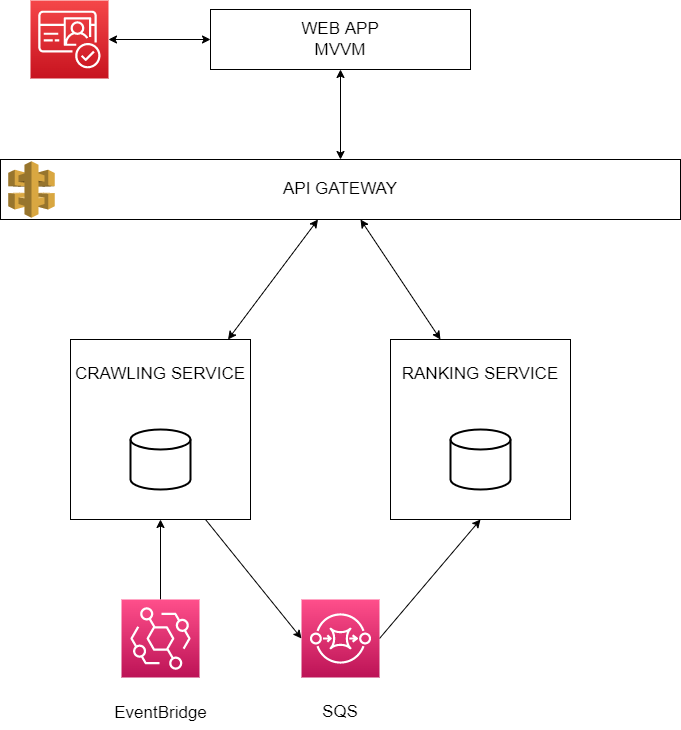
\includegraphics[scale=0.35]{Contenuto/Immagini/backend-architettura.png}
    \caption{Architettura generale}
\end{figure}

\subsubsection{Descrizione}
Come richiesto dal capitolato si è deciso di utilizzare un'architettura a microservizi, i quali comunicano con il Frontend tramite API Gateway\glo.
In particolare sono stati individuati i seguenti microservizi:
\begin{itemize}
    \item \textit{Crawling Service}: questo microservizio si occupa di tutto ciò che riguarda il crawling dei dati da Instagram. Il processo di crawling viene innescato da un servizio di AWS chiamato EventBridge\glo che si occupa dello scheduling del crawling. Ogni volte che viene trovato dal crawler un post relativo ad un ristorante, questo viene inviato ad una coda SQS\glo dalla quale andrà a leggere il servizio di ranking. Infine il Crawling Service espone una API al Frontend per permettere di suggerire profili Instagram da aggiungere alla lista di quelli osservati dal crawler.
    \item \textit{Ranking Service}: questo microservizio invece si occupa dell'analisi dei contenuti estratti dal crawler e della realizzazione di una classifica di ristoranti. Il processo di analisi di un post viene fatto partire dalla ricezione di un messaggio sulla coda SQS, una volta letto il messaggio esso viene rimosso dalla coda ed analizzato. Infine il Ranking Service espone molteplici API al Frontend in grado di fornire tutte le informazioni necessarie per poter visualizzare la classifica, i dettagli di un locale e la gestione dei preferiti.
\end{itemize}

Invece, per il Frontend è stato scelto di realizzare la struttura sfruttando il pattern architetturale \textit{Model-View-ViewModel} (MVVM), il quale comunica con il Backend esclusivamente tramite API Gateway.

Possiamo riassumere le motivazioni per cui abbiamo scelto il pattern architetturale MVVM per la parte Frontend come segue:

\begin{itemize}
\item La parte di Front-end è stata realizzata sfruttando la libreria React\glo che si integra particolarmente bene con il pattern MVVM,
\item Permette di riutilizzare i vari componenti in diversi contesti senza dover effettuare modifiche; un esempio è il modello che sfruttiamo per estrarre dati dal database, i quali (tramite la stessa chiamata) vengono usati in diverse pagine della WebApp. Lo stesso vale per la vista (perché usiamo un componente in diverse pagine della WebApp),
\item Permette di disaccoppiare la parte di business logic dalla presentation logic, aspetto che rende più semplice anche i test di unità,
\item Maggior semplicità di sviluppo in team: in questo modo, ogni singolo componente del gruppo può occuparsi di una sola parte della WebApp,
\item Manutenibilità più semplice, per via del disaccoppiamento del codice.
\end{itemize}
Inoltre, per la parte di autenticazione è stato utilizzato Cognito\glo, un servizio di AWS consigliatoci dall'azienda \textit{Zero12}, che permette di creare e gestire bacini d'utenza, oltre al framework AWS Amplify\glo per la parte di hosting ed autenticazione lato Frontend.


\subsubsection{Comunicazione tra servizi}
Per implementare la comunicazione tra il Crawling Service e Ranking Service viene utilizzata una coda SQS. La scelta di utilizzare il servizio SQS deriva da due motivi principali:
\begin{itemize}
\item Il servizio è completamente gestito da AWS, con un uptime del 99 \% ;
\item Si integra nativamente con il servizio Lambda\glo ;
\item Costi ridotti
\end{itemize}

\paragraph{Impostazioni coda SQS}
\'E stata scelta una coda di tipo \textbf{FIFO} poiché garantisce l'elaborazione unica di ogni messaggio e gestisce internamente i duplicati, cancellandoli. Questo viene a costo delle performance, che non sono una criticità poiché il servizio di analisi di Ranking Service lavora in background, consumando i messaggi ad una velocità ridotta.
Di seguito alcuni parametri impostati:
\begin{itemize}
\item \textbf{Visibility Timeout}: il tempo che un messaggio rimane nascosto dopo essere ricevuto da un consumatore. Impostato a 20 minuti poiché deve essere maggiore del tempo di esecuzione della Lambda che effettua l'analisi, che è di 15 minuti;
\item \textbf{Message retention period}: il tempo massimo di permanenza dei messaggi nella coda. Impostato a 2 giorni;
\item \textbf{Maximum message size}: La dimensione massima del messaggio. Impostata a 256 KB, che è la massima dimensione e quella consigliata da AWS.
\item \textbf{Receive message wait time}: Il tempo massimo che il consumatore aspetta per i messaggi che diventino disponibili. Impostata a 20 secondi, che è il tempo massimo. Questo riduce il consumo di risorse, perché aspetta 20 secondi prima di ritornare una risposta vuota e permette al consumatore di lavorare sempre a pieno regime, in quanto aspettando 20 secondi la coda generalmente fa in tempo a riempirsi di almeno un batch completo;
\item \textbf{Dimensione batch}: Il massimo numero di messaggi che un consumatore riceve per volta. Impostato a 10 che è il massimo per le code FIFO. In questo modo vengono ridotte le chiamate al servizio di analisi.
\end{itemize}

\paragraph{Dead letter queue}
Una dead letter queue (DLQ) è una coda agguntiva utilizzata per gestire i messaggi che non vengono elaborati con successo.
Il suo utilizzo si è ritenuto necessario per spostare della coda pricipale  i messaggi che generavano errori, permettendo a quelli corretti di essere elaborati, e quindi sbloccando la coda. Quindi i messaggi non corretti vengono spostati nella DLQ e possono essere analizzati in sede separata. I motivi principali per cui è stato scelto di usare una DLQ sono la semplificazione del testing e debug, permettendo di mantenere il servizio in funzione e la possibilità di reindirizzare nella coda principale i messaggi che generavano errore (dopo che il problema è stato individuato e risolto) evitando di perderli.
Di seguito alcuni dei parametri impostati:
\begin{itemize}
\item \textbf{Message retention period}: Impostato al suo valore massimo, 14 giorni, così da far pemanere più tempo possibile i messaggi che generano errore;
\item \textbf{Maximum Receives}:  Il numero massimo di volte che il messaggio viene ricevuto ed elaborato senza successo. Impostato a 3, quindi dopo la seconda elaborazione senza successo viene messo nella DLQ. Il valore è stato deciso empiricamente, in questo modo i messaggi vengono ritentati per 3 volte nel giro di un'ora (20 minuti di visibility timeout). L'idea è che in generale un eventuale problema di downtime di qualche servizio possa essere mitigato e al tempo stesso si evita di riprovare troppe volte un messaggio che genera errore nel codice delle procedure, poiché finché non viene corretto, verrà continuamente generato lo stesso errore, sprecando risorse ed impedendo ad eventuali altri messaggi corretti di venire elaborati. 
\end{itemize}
In generale il resto delle impostazioni resta identico a quello della coda principale.

